\chapter{Modellazione del sistema}
\label{cap:modelling}
Il modello realizzato offre le funzionalità sopra descritte implementando un
sistema di \textit{Interlocking Distribuito} di nodi di tracciati e treni.
\section{Tracciato e itinerari}
Il tracciato relativo al nostro progetto è composto da:
\begin{itemize}
  \item cinque Circuiti di Binario (GA1, GA2, GA3, GA4, GA5) di cui 
  \begin{itemize}
    \item GA1 e GA4 sono \textit{outer\_station},
    \item GA5 è associato a un binario morto;
	\end{itemize}
	\item tre locazioni di scambio (W1, W2, W3);
	\item sette semafori
	\begin{itemize}
	  \item A per le segnalazioni nella direzione GA1-\textgreater W1,
	  \item P1 per le segnalazioni nella direzione GA2-\textgreater W1,
	  \item P2 per le segnalazioni nella direzione GA3-\textgreater W1,
	  \item N2 per le segnalazioni nella direzione GA2-\textgreater W2,
	  \item N3 per le segnalazioni nella direzione GA3-\textgreater W3,
	  \item F per le segnalazioni nella direzione GA4-\textgreater W2,
	  \item S10 per controllare l'uscita dal binario morto GA5.
	 \end{itemize} 
\end{itemize}

\begin{figure}
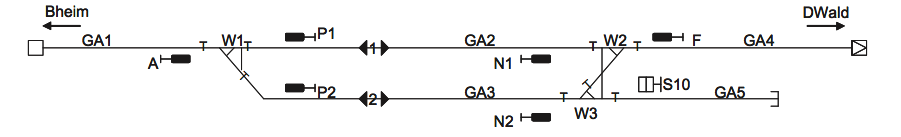
\includegraphics[width=13.5cm]{imgs/reteInterlocking.png}
\caption{Tracciato ferroviario utilizzato per la simulazione}\label{fig:X}
\end{figure}



Nel tracciato illustrato sono possibili i seguenti itinerari:
\begin{enumerate}
  \item GA1 A W1 GA2
  \item GA1 A W1 GA2 N1 W2 GA4
  \item GA1 A W1 GA3
  \item GA1 A W1 GA3 N2 W3 W2 GA4
  \item GA1 A W1 GA3 N2 W3 GA5
  \item GA4 F W2 GA2
  \item GA4 F W2 GA2 P1 W1 GA1
  \item GA4 F W2 W3 GA3
  \item GA4 F W2 W3 GA3 P2 W1 GA1
  \item GA5 S10 W3 GA3
  \item GA2 P1 W1 GA1
  \item GA2 N1 W2 GA4
  \item GA3 P2 W1 GA1
  \item GA3 N2 W3 W2 GA4
  \item GA3 N2 W3 GA5
\end{enumerate}

\section{Modello del Circuito di Binario}
Il Circuito di Binario è modellato con la classe \textit{TrackCircuit} la quale
è a conoscenza dei Circuiti di Binario precedenti e successivi (variabili
\textit{prev} e \textit{next}) per ogni possibile itinerario, sa istantaneamente
se è presente un treno (varibile \textit{train}), inoltre utilizza la variabile
booleana \textit{outer\_station} per sapere se è una stazione esterna nel
tracciato considerato. Tutte queste varibili vanno assegnate in fase di creazione di ogni
singolo oggetto.

Il comportamento dinamico del \textit{TrackCircuit} è rappresentato nella figura
\ref{fig:Circuito} dove sono evidenziati sia gli stati in cui un Circuito di Binario
può trovarsi sia quali segnali permettono le trasizioni.

\begin{sidewaysfigure}

\centering
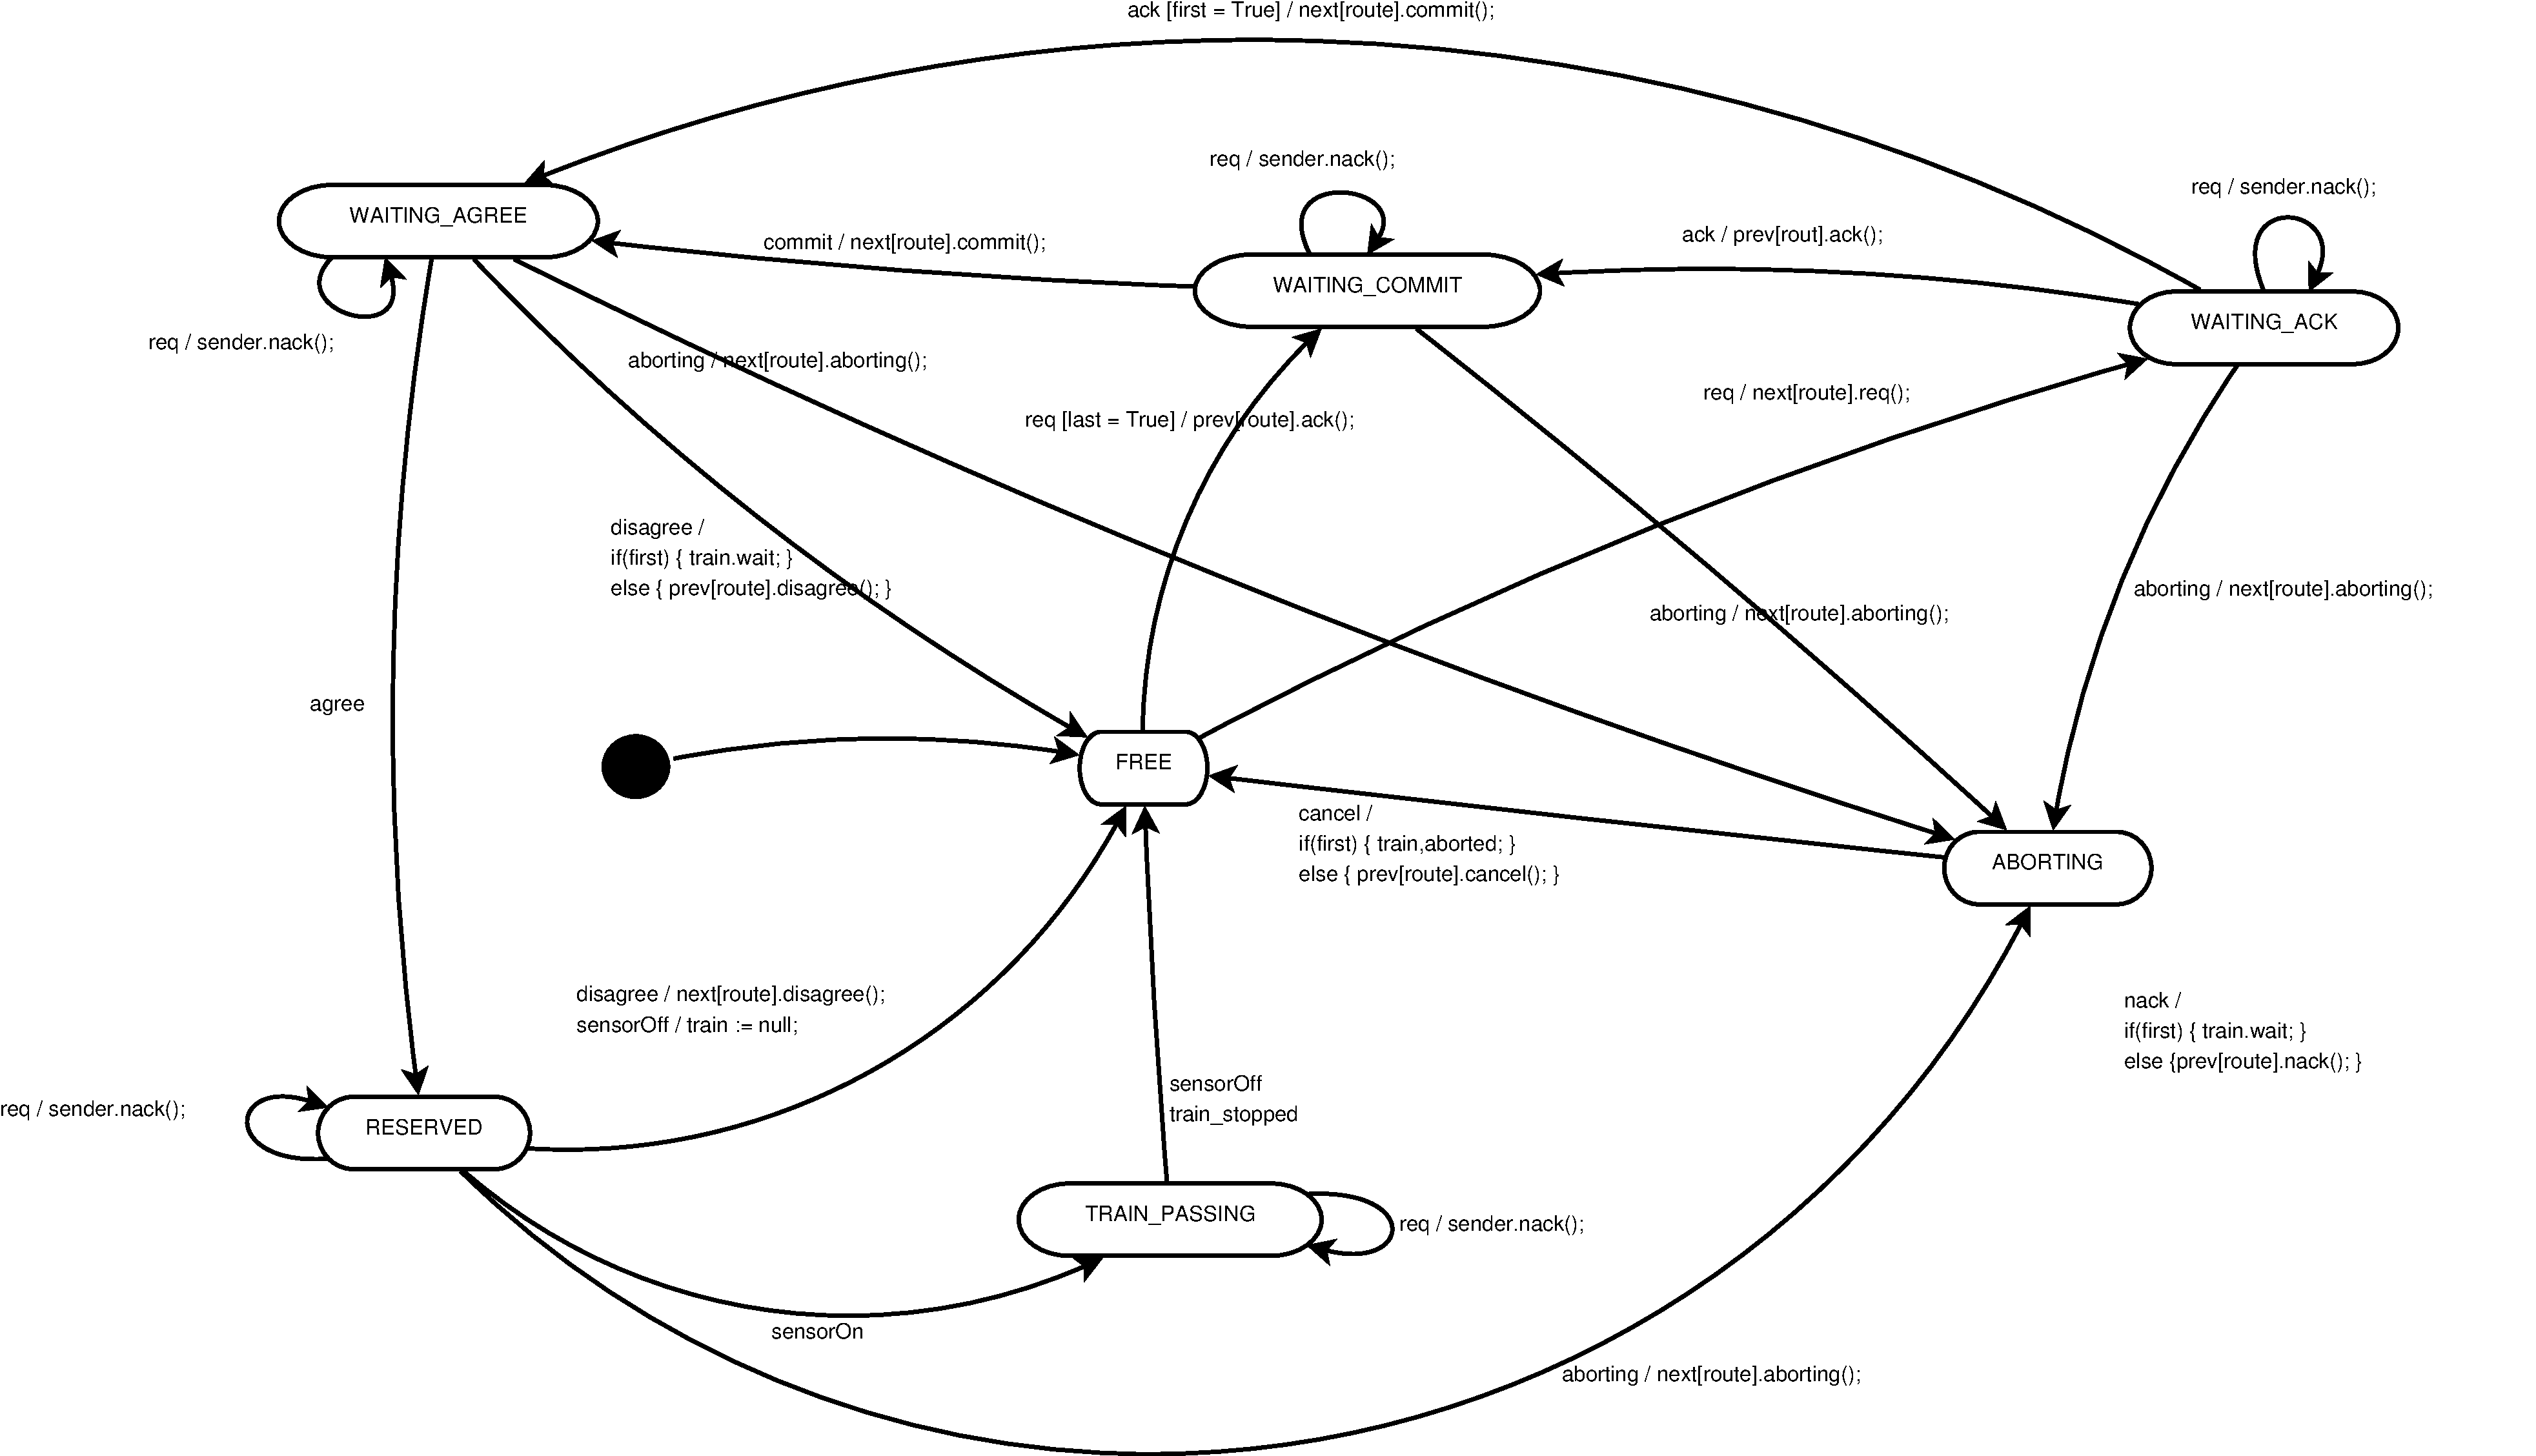
\includegraphics[width=24cm]{imgs/TrackCircuit.pdf}

\caption{Diagramma di variazione degli stati del Circuito
di Binario}\label{fig:Circuito}

\end{sidewaysfigure}



I segnali che possono essere elaborati dal \textit{TrackCircuit} sono:
\begin{itemize}
\item \textbf{Request} Il segnale \textit{req(sender, dest, route)} indica una
richiesta di prenotazione per l’itinerario route da parte dell’oggetto
\textit{sender} (un Treno, uno Scambio oppure un altro Circuito di Binario).
Quando viene ricevuto può essere rifiutato qualora lo stato corrente non sia
FREE rispondendo con un segnale \textit{nack} (o col segnale \textit{wait} se è
il primo nodo dell’itinerario), oppure può essere accettato
eseguendo la transizione nello stato \textit{WAITING\_ACK} e propagando la
richiesta al nodo successivo dell’itinerario. Se ci troviamo sul nodo finale lo
stato diverrà \textit{WAITING\_COMMIT} e non viene propagato nessun messaggio,
ma si risponde al mittente con un messaggio di \textit{ack}.

\item \textbf{Acknowledgement} Il segnale \textit{ack(sender, dest, route)} indica un
riscontro positivo alla richiesta di prenotazione relativo all’itinerario route da parte
dell’oggetto sender. Un nodo che riceve questo messaggio ha precedentemente
propagato un messaggio di req e si trova nello stato \textit{WAITING\_ACK},
quindi propaga l’ack al nodo precedente sull’itinerario e si pone in attesa del
\textit{commit} eseguendo la transizione allo stato \textit{WAITING\_COMMIT}. Se
a ricevere l’\textit{ack} è il primo nodo dell’itinerario questo si porta
direttamente nello stato \textit{WAITING\_AGREE} e spedisce un messaggio di
\textit{commit} in avanti.

\item \textbf{Negative Acknowledgement} Il segnale \textit{nack(sender, dest, route)}
rappresenta un riscontro negativo alla richiesta di prenotazione per l’itinerario route da parte
dell’oggetto sender. Un nodo che riceve questo messaggio ha precedentemente
propagato un messaggio req e poiché la prima fase del 2PC è fallita, propaga il
nack al nodo precedente sull’itinerario e ritorna allo stato FREE in attesa di una
nuova richiesta di prenotazione.

\item \textbf{Commit} Il segnale \textit{commit(sender, dest, route)} indica un
commando di “conferma prenotazione” per l’itinerario route inoltrata dall’oggetto sender. Un nodo
che riceve questo messaggio ha precedentemente propagato i messaggi req e ack
dunque si trova in \textit{WAITING\_COMMIT} e alla sua ricezione lo propaga al
nodo successivo e si pone nello stato \textit{WAITING\_AGREE}. Se il nodo è
l’ultimo dell’itinerario invece che inoltrare il \textit{commit} spedisce
indietro un messaggio \textit{agree} e si porta direttamente in
\textit{RESERVED} in attesa che il treno vi transiti sopra.

\item \textbf{Agree} Il segnale \textit{agree(sender, dest, route)} indica la
prenotazione finale per l’itinerario route da parte dell’oggetto sender. Un nodo che riceve questo messaggio
ha precedentemente propagato i messaggi \textit{req, ack e commit} quindi alla
ricezione dell’\textit{agree} lo propaga al nodo precedente sull’itinerario (o
invia uno start al treno se è il primo nodo dell’itinerario) e si pone nello
stato \textit{RESERVED}.

\item \textbf{Disagree} Il segnale \textit{disagree(sender, dest, route)} indica il
fallimento di un \textit{commit} per l’itinerario route. Nel nostro modello solo
uno Scambio può sollevare il fallimento del \textit{commit} quindi un Circuito
di Binario può solo riceverlo. In tal caso, se si trova nello stato \textit{WAITING\_AGREE}, lo propaga al nodo precedente, se invece si trova nello stato \textit{RESERVED} allora lo propaga al nodo successivo. In
entrambi i casi, dopo l’inoltro, si porta allo stato \textit{FREE}. La
differenza di comportamento in base allo stato corrente è dovuta al fatto che il
\textit{disagree} è spedito da uno Scambio in entrambe le direzioni, quindi se il Circuito di Binario lo riceve dal nodo successivo vuol dire che ancora non ha ricevuto un \textit{agree}, quindi si trova in
\textit{WAITING\_AGREE} e deve inoltrarlo indietro, se invece lo riceve dal nodo precedente,
allora vuol dire che ha già fatto passare un agree ed è quindi riservato, dunque
dovrà inoltrare il \textit{disagree} in avanti.

\item \textbf{Abort} Il segnale \textit{aborting(sender, dest, route)} indica la
richiesta di cancellazione dell’itinerario route per il quale era stata precedentemente inviata una
richiesta di prenotazione. Il primo messaggio di questa richiesta parte sempre
da un treno e ogni Circuito di Binario, alla ricezione di tale messaggio, inoltra
la richiesta al nodo successivo e si porta nello stato \textit{ABORTING}.
Qual’ora il nodo sia l’ultimo dell’itinerario allora passa direttamente allo
stato \textit{FREE} e spedisce indietro un messaggio di \textit{cancel}.

\item \textbf{Cancel} Il segnale \textit{cancel(sender, dest, route)} indica la
conferma di cancellazione dell’itinerario route. Alla ricezione di questo messaggio un Circuito di Binario
inoltra la richiesta al nodo precedente lungo l’itinerario e si porta nello stato
\textit{FREE} tornando ad essere libero e in attesa di una nuova prenotazione.
Qual’ora il circuito sia quello su cui si trova il treno che ha richiesto la cancellazione allora,
oltre ad eseguire la trasizione verso lo stato \textit{FREE} spedisce il
messaggio \textit{aborted} al treno. In questa situazione l’itinerario è stato
reso tutto libero e il treno può e chiedere una nuova prenotazione.

\item \textbf{Wait} Il segnale \textit{wait} viene ricevuto se sull'itinerario qualche
nodo ha avuto un fallimento. Il treno per mantenere la proprietà del
sistema commuta il suo stato in \textit{CANCELLED}.
\end{itemize}

Gli stati in cui può trovarsi un TrackCircuit sono:
\begin{itemize}
  \item \textbf{FREE}: il circuito è libero in attesa di una prenotazione;
  \item \textbf{WAITING\_ACK}: ha ricevuto il messaggio \textit{req} ed è in
  attesa di un \textit{ack} (questo stato e non è possibile per l’ultimo nodo di ogni
  itinerario);
  \item \textbf{WAITING\_COMMIT}: ha ricevuto il \textit{ack} e lo ha inoltrato,
  quindi è in attesa di un \textit{commit} (questo stato non è permesso al primo
  nodo dell’itinerario);
  \item \textbf{WAITING\_AGREE}: ha ricevuto il commit e lo ha inoltrato, quindi
  è in attesa di un \textit{agree} (questo stato non è permesso all’ultimo nodo
  dell’itinerario);
  \item \textbf{RESERVED}: il circuito è riservato ed è in attesa del transito
  del treno;
  \item \textbf{TRAIN\_PASSING}: un treno si trova sul circuito;
  \item \textbf{ABORTING}: il circuito ha ricevuto un messaggio di aborting ed è
  in attesa di ricevere il \textit{cancel}.
  \item \textbf{CANCELLED}: il treno non ha avuto riscontro positivo per il
  fallimento di qualche nodo sul tracciato. L'inserimento di questo stato
  facilita l'analizzabilità del modello. 
\end{itemize}

\section{Modello dello Scambio}
Lo Scambio viene modellato con la classe \textit{Switch} rappresentata con i
suoi stati e transizioni nella figura \ref{fig:Scambio}.
\begin{sidewaysfigure}

\centering
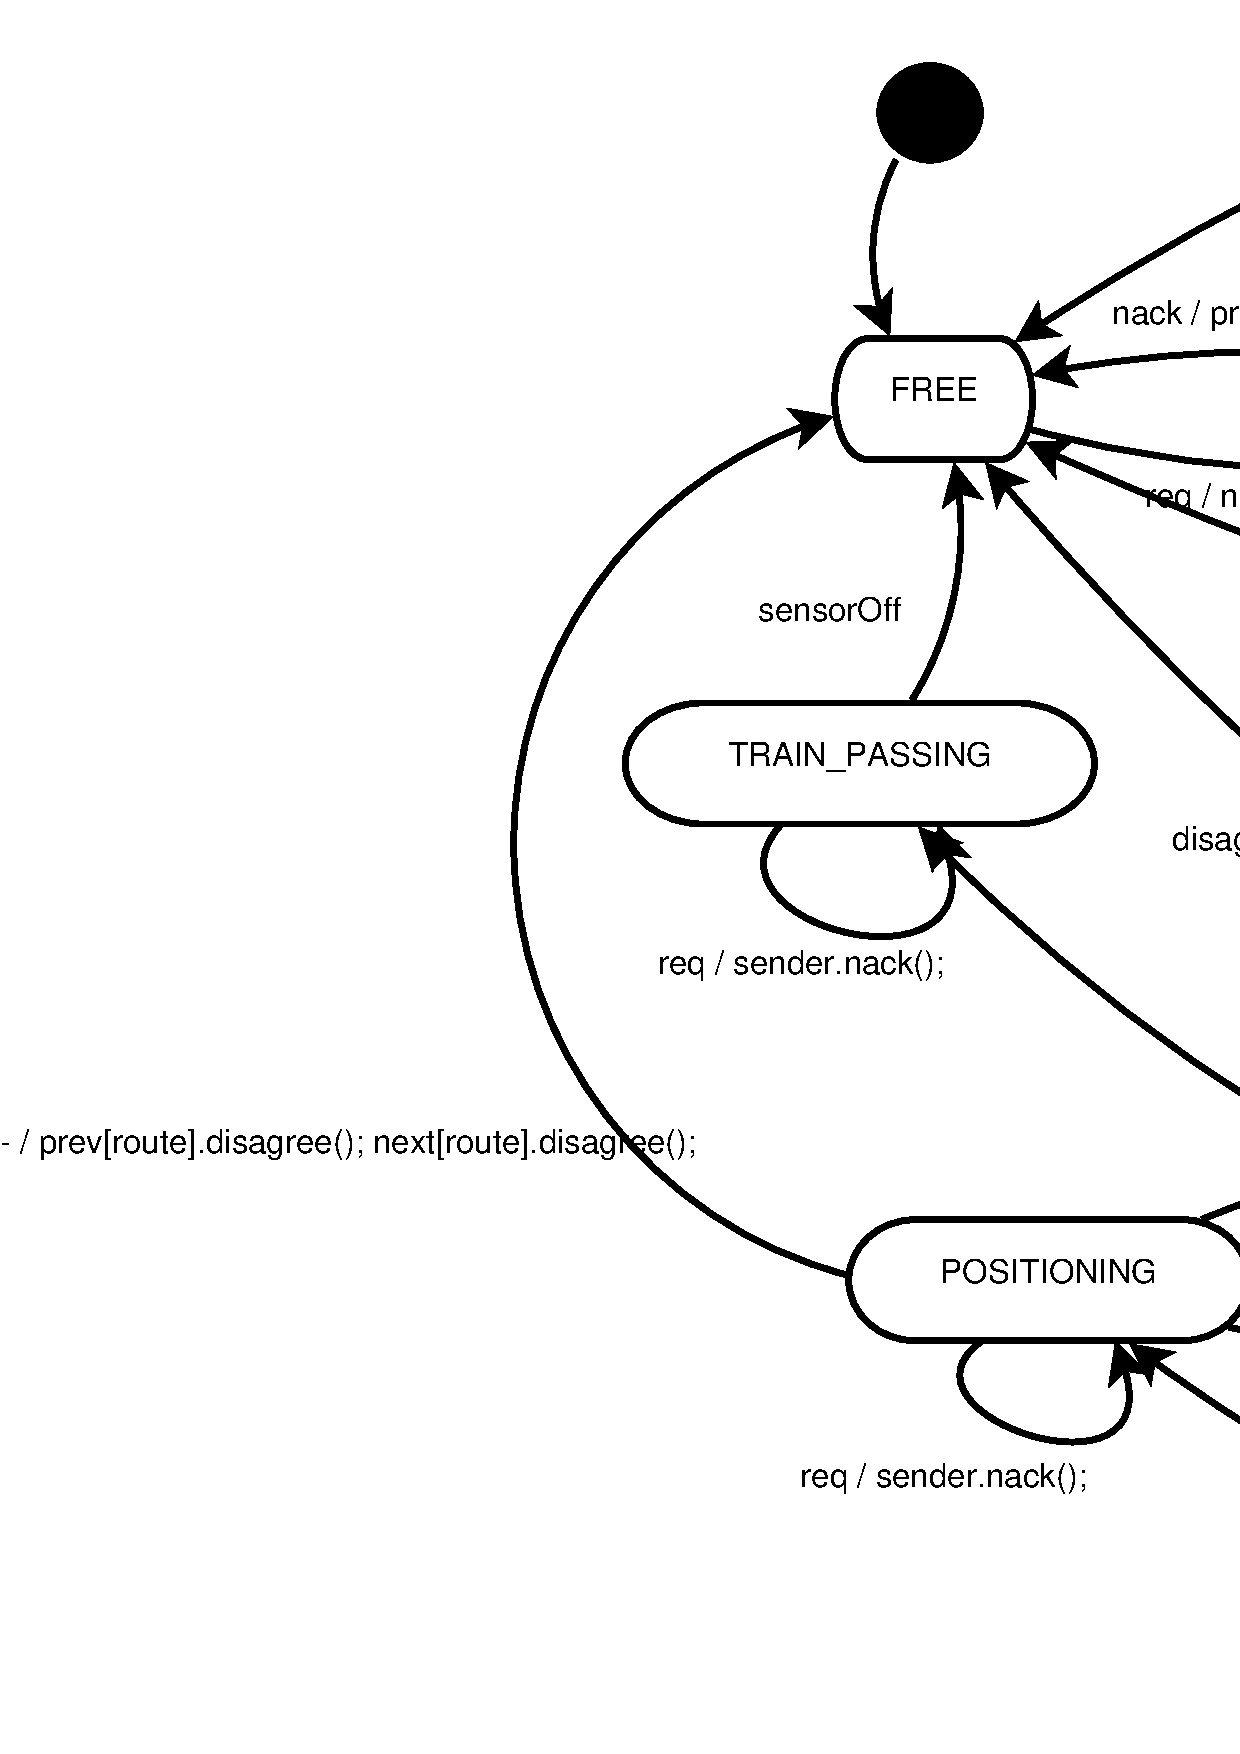
\includegraphics[width=24cm]{imgs/Switch.pdf}

\caption{Diagramma di variazione degli stati dello Scambio}\label{fig:Scambio}

\end{sidewaysfigure}

L’algoritmo di prenotazione implementato da questa classe è lo stesso di quello
della classe \textit{TrackCircuit} con alcune varianti dovute al fatto che:
\begin{enumerate}
  \item uno Scambio non può mai essere il primo o l’ultimo nodo di un itinerario,
quindi i messaggi possono essere solo ricevuti e spediti a Circuiti di Binario o
altri Scambi, mai a treni, di conseguenza non sono presenti salti in avanti da
\textit{FREE} a \textit{WAITING\_COMMIT} e da \textit{WAITING\_COMMIT} a
\textit{RESERVED}, o da \textit{WAITING\_ACK} a \textit{WAITING\_AGREE} propri
dei Circuiti di Binario iniziali e finali;
\item i treni non possono fermarsi su uno Scambio, quindi la richiesta di
 cancellazione di un itinerario non può avvenire su uno Scambio;
\item gli Scambi devono posizionarsi prima di permettere il passaggio del treno
(il posizionamento può fallire, ed è in questo caso che viene spedito un messaggio
di \textit{disagree}). 
\end{enumerate}

Ogni oggetto della classe \textit{Switch} ha due variabili aggiuntive rispetto
ai Circuiti di Binario, ossia \textit{reversed} e \textit{conf} che
rappresentano, rispettivamente, il posizionamento corrente (normale o rovescio)
e quale deve essere il posizionmento corretto per ogni itinerario. Per
permettere il posizionamento sono stati implementati due stati aggiuntivi,
\textit{CHECK\_POSITION e POSITIONING}, il loro ruolo è il seguente:
\begin{itemize}
  \item \textbf{CHECK\_POSITION}: lo Scambio si sposta in questo stato subito
  dopo aver ricevuto un agree e controlla se il suo posizionamento è corretto
  per l’itinerario richiesto (ossia se reversed == conf[route]). Se il
  posizionamento è giusto inoltra il messaggio \textit{agree} e si porta in
  \textbf{RESERVED} in attesa del transito del treno, se il posizionamento
  invece non è corretto allora passa allo stato \textit{POSITIONING};
  \item \textbf{POSITIONING}: in questo stato si aggiusta il posizionamento dello
	Scambio. Tale operazione può fallire, ossia non deterministicamente invece che
	passare allo stato \textit{RESERVED} inoltrando l’\textit{agree}, passa allo
	stato \textit{FREE} spedendo in entrambe le direzioni un \textit{disagree} che
	viene propagato su tutto l’itinerario cancellando, di fatto, la prenotazione.
\end{itemize}

\section{Modello del treno}
Il treno è stato implementato nella classe \textit{Train} rappresentata in
figura \ref{fig:Treno}.
\begin{sidewaysfigure}

\centering
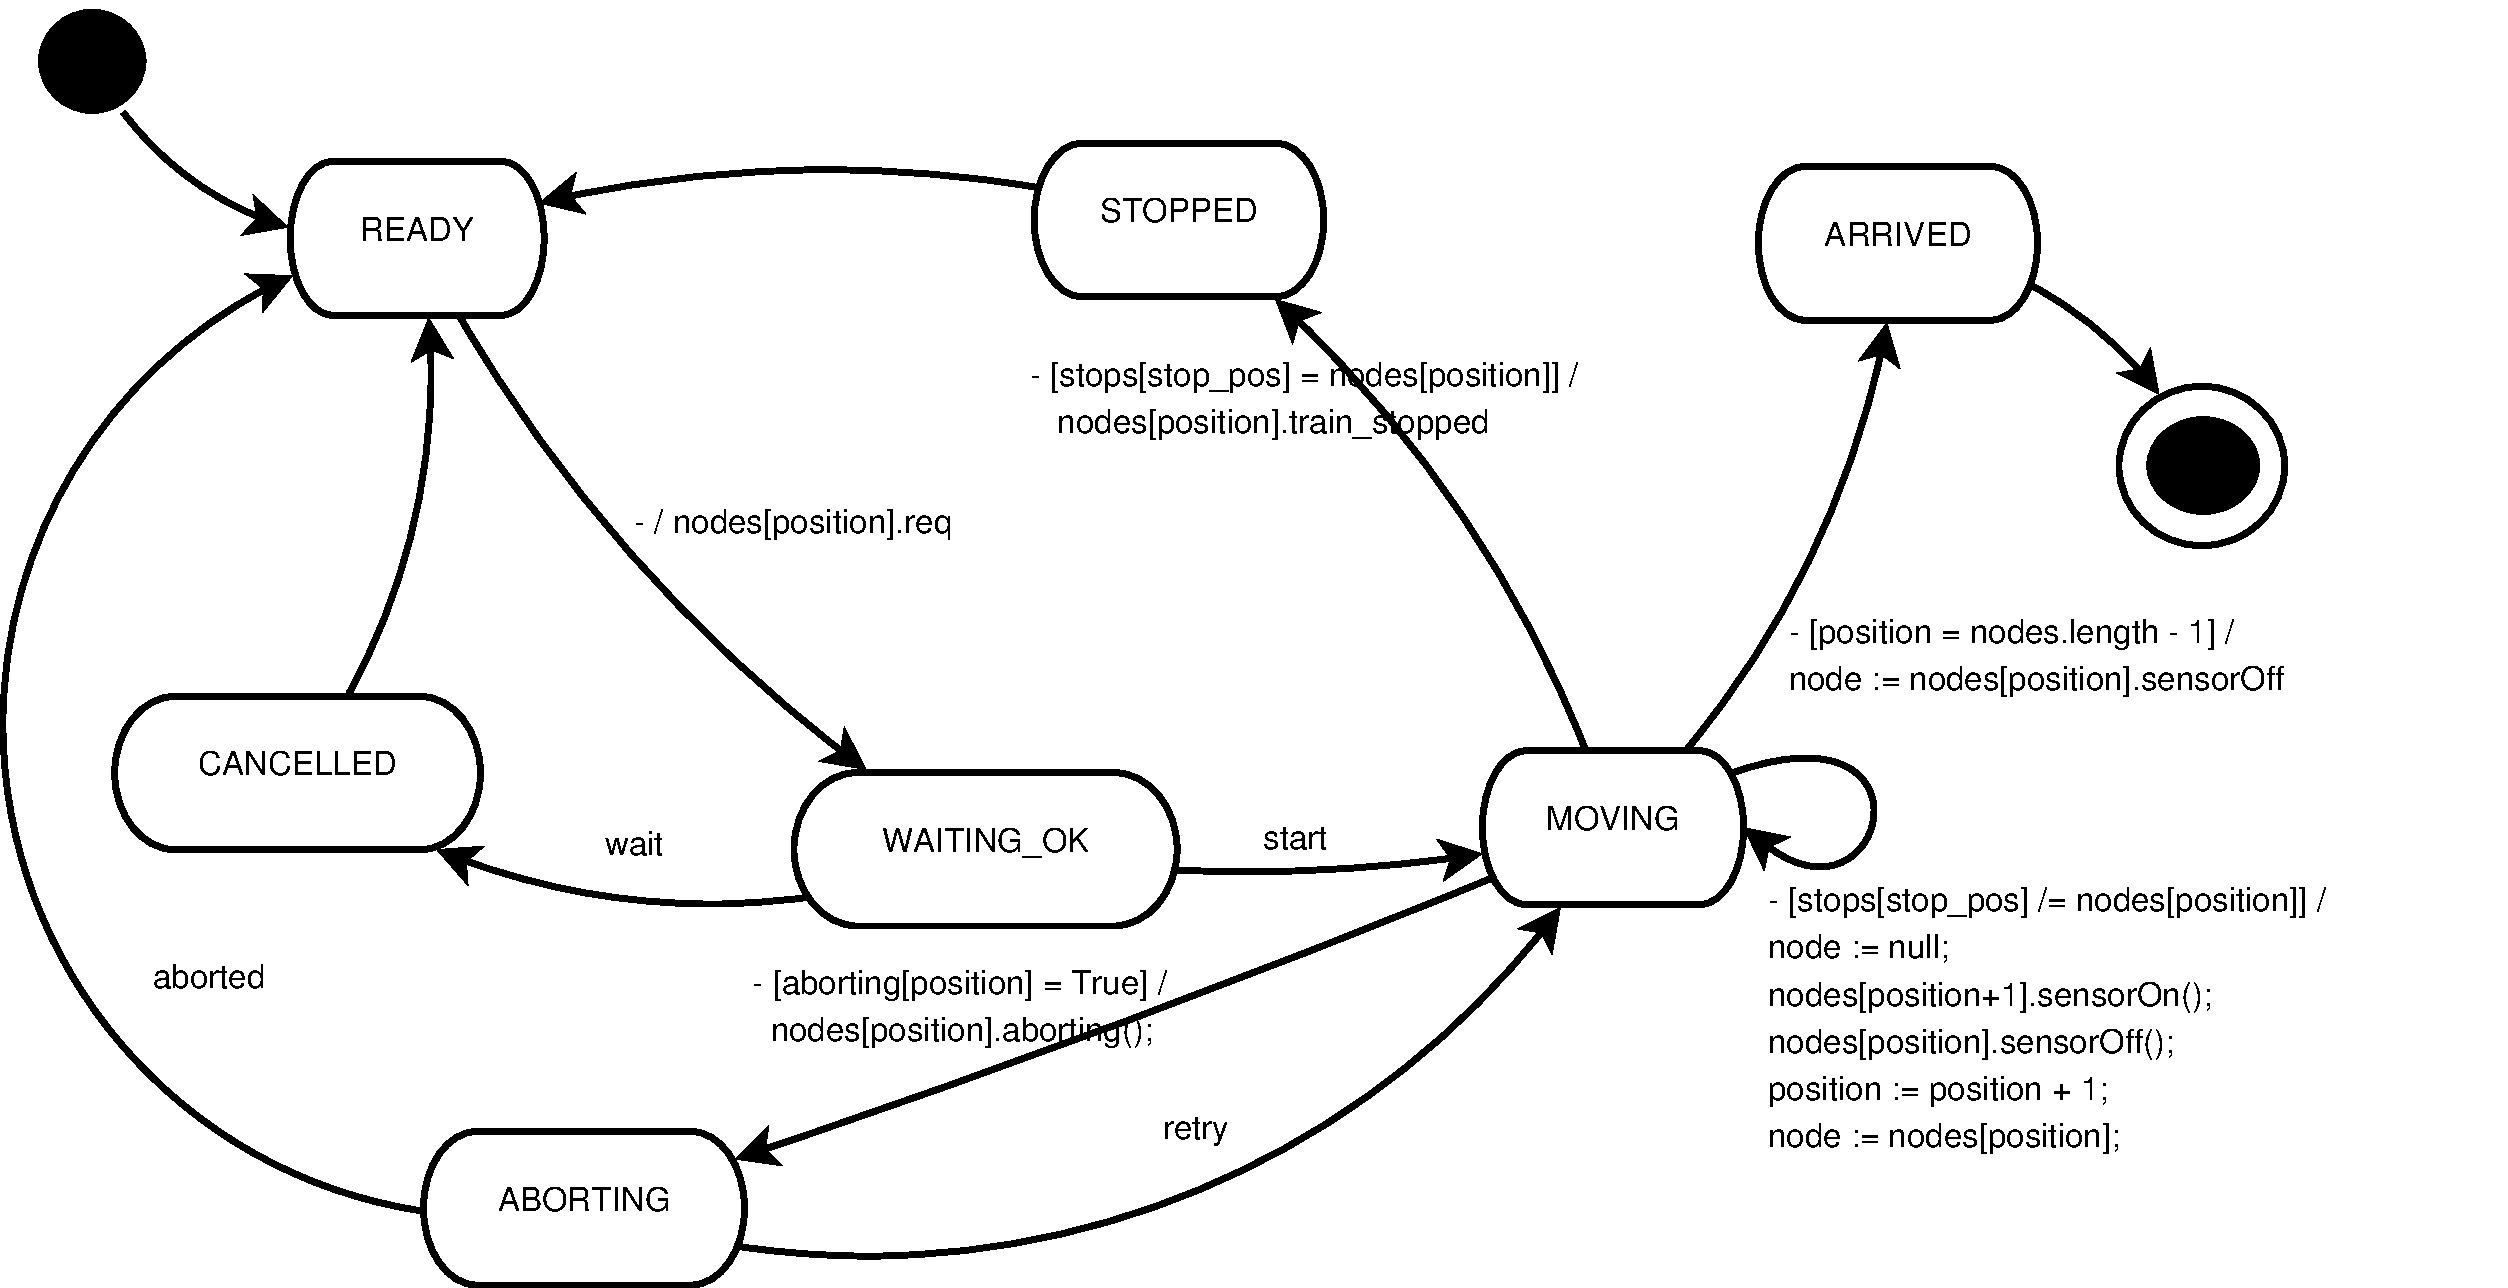
\includegraphics[width=24cm]{imgs/Train.pdf}

\caption{Diagramma di variazione degli stati del Treno}\label{fig:Treno}

\end{sidewaysfigure}

Il suo compito è quello di richiedere un itinerario inviando al Circuito di
Binario sul quale si trova un messaggio di \textit{req}. Se la prenotazione ha
successo, e quindi riceve in risposta un messaggio di \textit{start}, si muove
di nodo in nodo fino a raggiungere l’ultima stazione. A questo punto può
chiedere un nuovo itinerario oppure uscire dal tracciato, qual’ora si sia
fermato su un nodo esterno (ossia un Circuito di Binario in cui la variabile
\textit{outer\_station} == True).
In fase di istanziazione, ad ogni oggetto della classe \textit{Train} sono
assegnati:
\begin{itemize}
  \item un vettore di interi routes, rappresentante gli itinerari che il treno
  deve percorrere prima di fermarsi; 
  \item un vettore (nodes) contenente i nodi che compongono tutti gli
  itinerari da percorrere (tale vettore viene utilizzato durante la fase di
  movimento per sapere qual è il successivo nodo verso cui muoversi);
  \item un vettore di stazioni (stops) che indica su quali Circuiti di Binario
  il treno deve fermarsi;
  \item un vettore di nodi (aborting) che contiene i nodi sui quali il treno
  simula un malfunzionamente e invia la richiesta di cancellazione dell’itinerario.
\end{itemize}
Nella fase iniziale, il treno cicla fra gli stati \textit{READY} ed
\textit{WAITING\_OK} fino a quando non riceve una conferma positiva (messaggio
start) alla richiesta di prenotazione del primo itinerario. Se la prenotazione
non è andata a buon fine, ossia un nodo risulta già prenotato da un altro treno,
il messaggio di ritorno sarà un \textit{wait} e quindi il treno si riporta nello
stato \textit{CANCELLED} e, successivamente, nello stato \textit{READY} in attesa di tentare una nuova prenotazione.
Durante il movimento il treno si sposta da un nodo al successivo inviando messaggi
di sensorOn al nodo su cui entra e sensorOff al nodo dal quale esce. La chiamata
a \textit{sensorOff} di fatto riporta il nodo di uscita nello stato
\textit{FREE} rendendolo disponibile per una nuova prenotazione.
Quando il treno giunge alla fine di un itinerario segnalerà la fermata al
Circuito di Binario sul quale si trova per mezzo di un messaggio
\textit{train\_stopped} e torna nello stato \textit{READY} pronto per inviare la
richiesta di prenotazione per l’itinerario successivo.Se siamo giunti alla fine
dell’ultimo itinerario e la stazione è un nodo esterno il messaggio 
di \textit{sensorOff} permetterà anche l’uscita del treno dall’intero tracciato.

\section{Modello del Semaforo}
Il semaforo viene modellato con la classe \textit{Semaphore} rappresentata il cui diagramma di stato è in figura \ref{fig:semaforo}.
\begin{sidewaysfigure}

\centering
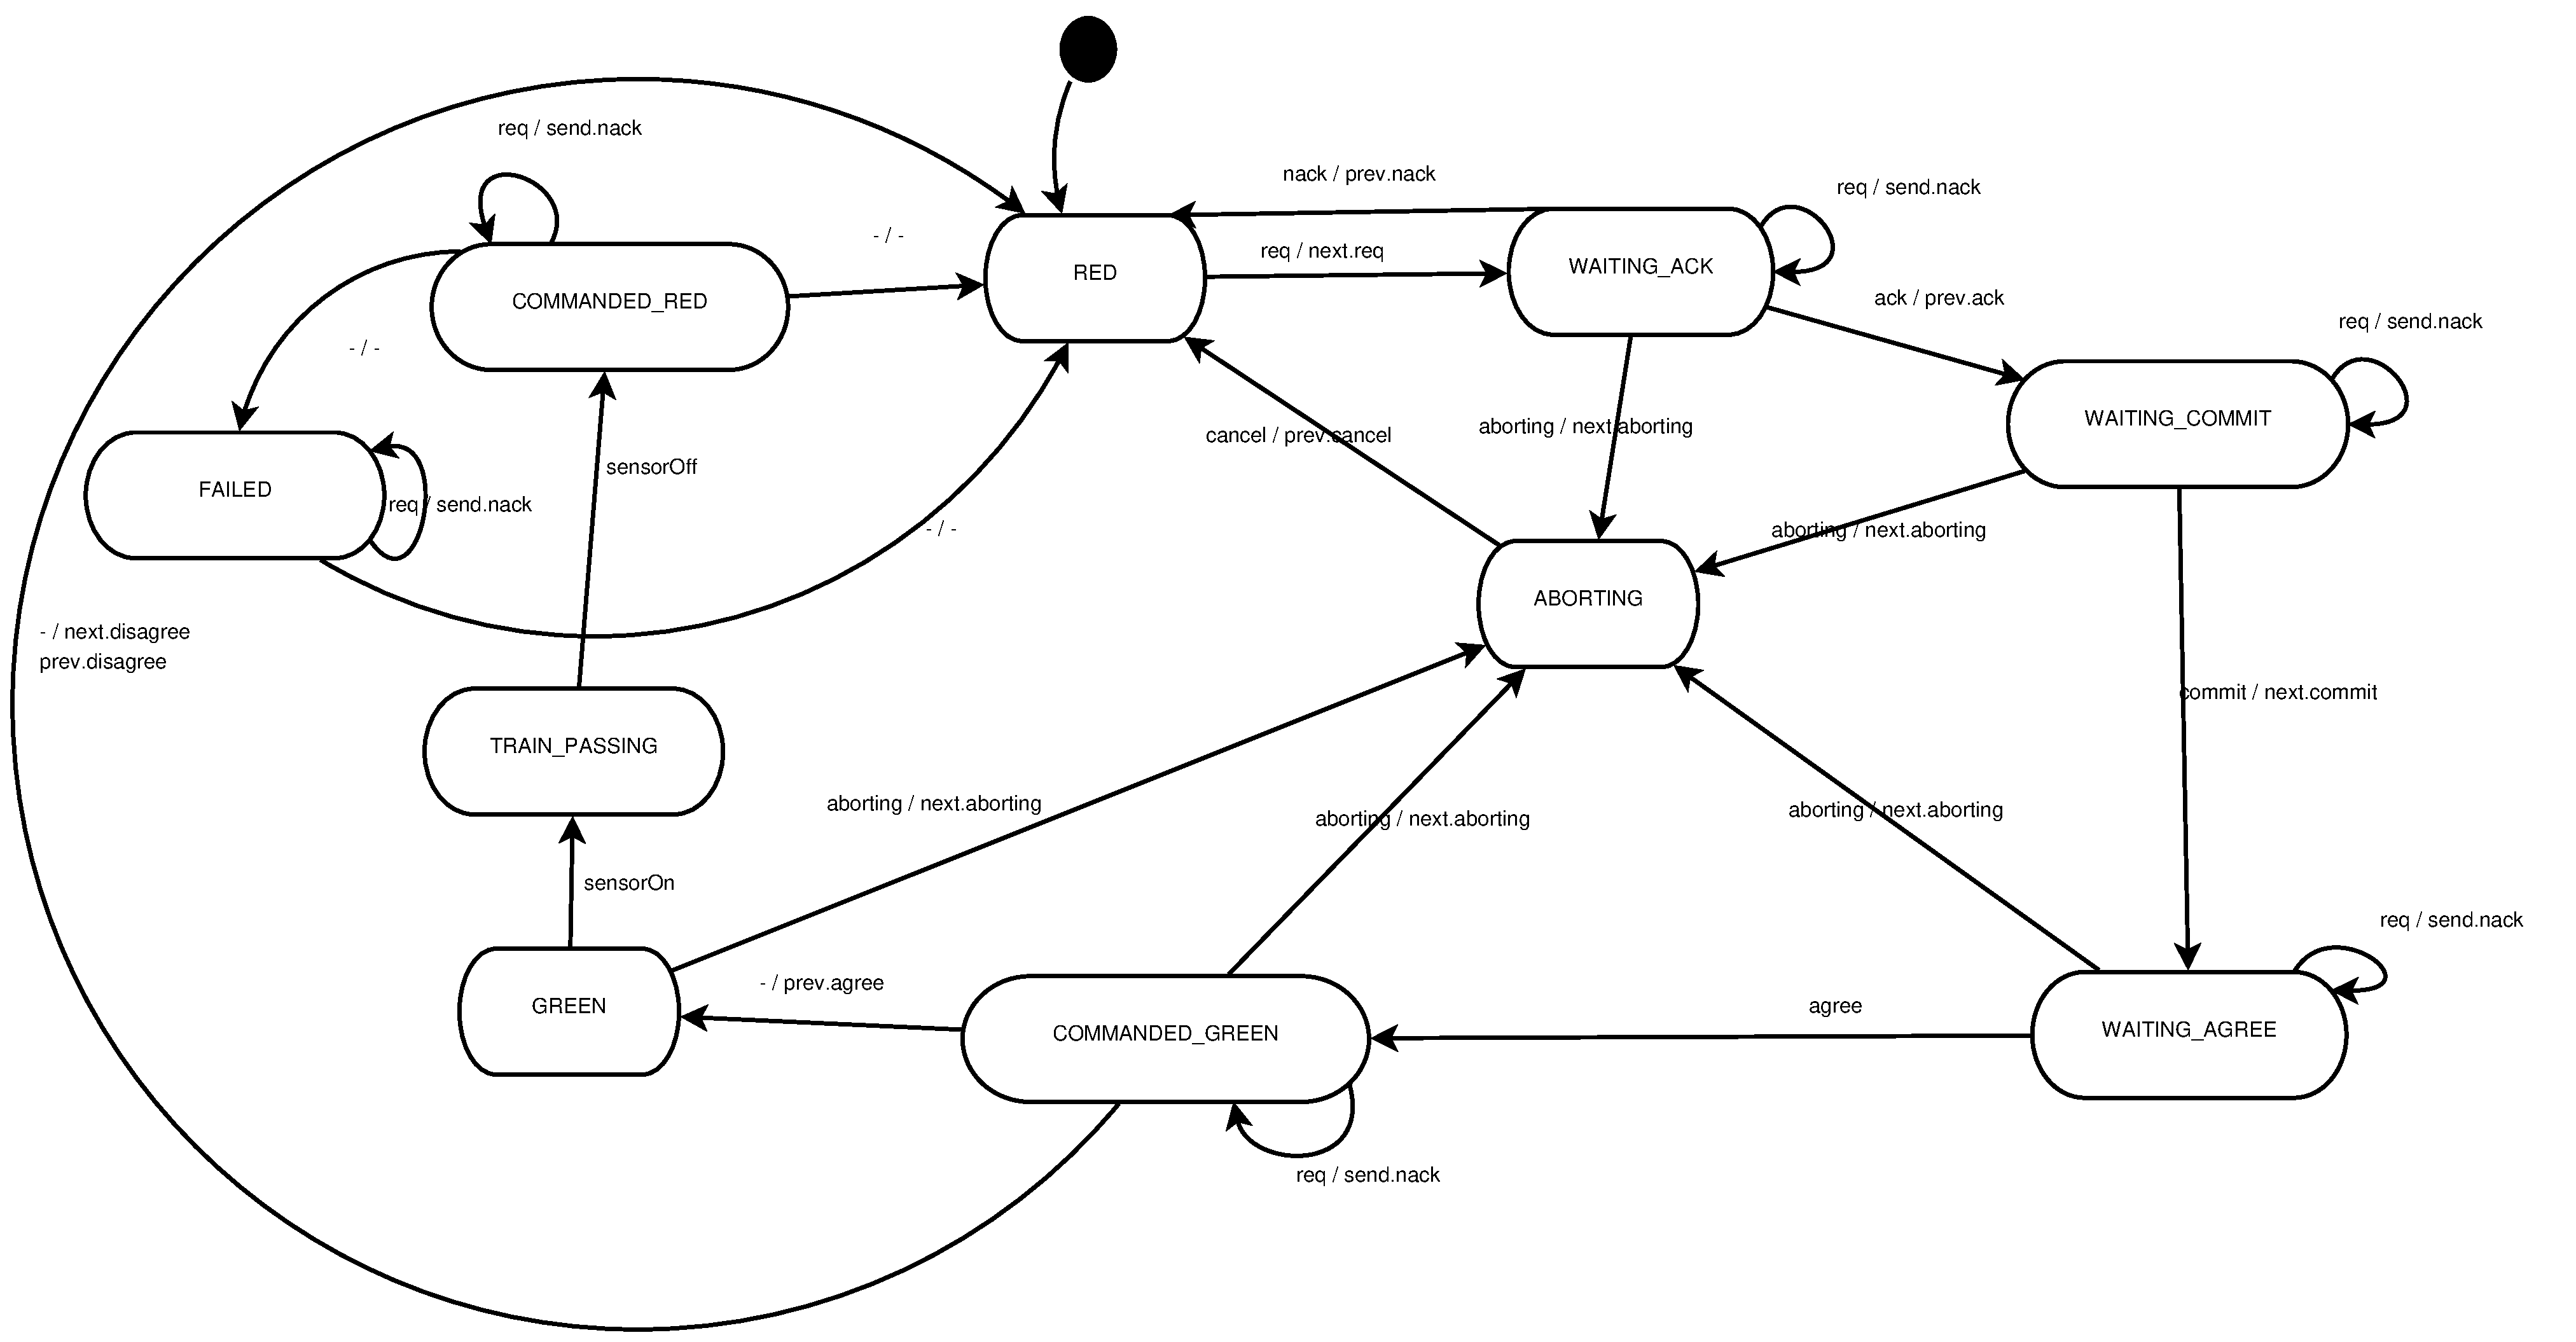
\includegraphics[width=24cm]{imgs/Semaphore.eps}

\caption{Diagramma di variazione degli stati del Semaforo}\label{fig:semaforo}

\end{sidewaysfigure}

Il semaforo, per la semantica della rete, non può essere il termine di un
itinerario, quindi ha all'interno dell'algoritmo di prenotazione solo
responsabilità di ricezione e inoltro dei segnali in arrivo e variazione del
proprio stato. La commutazione del segnale proposto è soggetta a fallimenti.

I segnali elaborati dal \textit{Semaphore} sono:
\begin{itemize}
  \item \textbf{Request} Il segnale \textit{req} dà inizio alla procedura per la prenotazione del nodo. Viene accettato
  e inoltrato al nodo successivo se lo stato del semaforo è \textit{RED}
  commutandolo in \textit{WAITING\_ACK}. La ricezione della
  \textit{request} in qualsiasi altro stato genera una risposta negativa attraverso il segnale
  \textit{nack}.
  \item \textbf{Acknowledgement} Il segnale \textit{ack} indica un riscontro posivito della richiesta di prenotazione da
  parte dei successivi nodi dell'itinerario. Il compito del semaforo è
  propagare il segnale e porre il suo stato in \textit{WAITING\_COMMIT}.
  \item \textbf{Negative Acknowledgement} Rappresentato dal
  segnale\textit{nack} indica un rifiuto della richiesta di prenotazione da parte dei successivi nodi
  dell'itinerario. Il semaforo propaga il \textit{nack} verso il \textit{Circuito di Binario} dove
  risiede il treno richiedente e ritorna nel suo stato iniziale \textit{RED}.
  \item \textbf{Commit} Il segnale \textit{commit} rappresenta il comando di conferma prenotazione inviata dal treno. Il
  semaforo propaga il segnale e si pone nello stato \textit{WAITING\_AGREE}
  \item \textbf{Agree} Il segnale \textit{agree} rappresenta il segnale finale della procura \emph{2PC}. Il semaforo che
  riceve questo segnale prima di inoltrarlo al nodo precedente dell'itinerario
  cambia il suo stato in \textit{COMMANDED\_GREEN}.
  \item \textbf{Abort} \textit{aborting} è il segnale per comunicare ai nodi dell'itinerario il
  fallimento del treno. I nodi, ed in particolare il semaforo, si pongono nello stato
  \textit{ABORTING}.
  \item \textbf{Cancel} \textit{cancel} è il segnale di conferma della ricezione di \textit{aborting} da parte dell'itinerario successivo al semaforo.
  Nel caso del semaforo comporta il passaggio di stato a \textit{RED}.
\end{itemize}

Gli stati possibili della classe \textit{Semaphore} sono:
\begin{itemize}
  \item \textbf{RED} Lo stato di attesa per la prenotazione.
  \item \textbf{WAITING\_ACK} ha ricevuto la richiesta ed è in attesa di
  \textit{ack}.
  \item \textbf{WAITING\_COMMIT} ha ricevuto l'\textit{ack} e lo ha inoltrato,
  quindi è in attesa di un \textit{commit}. 
  \item \textbf{WAITING\_AGREE} ha ricevuto il \textit{commit} e lo ha
  inoltrato, quindi è in attesa di un \textit{agree}. 
  \item \textbf{TRAIN\_PASSING} un treno si trova sul semaforo.
  \item \textbf{ABORTING} il semaforo ha ricevuto un messaggio di
  \textit{aborting} ed è in attesa di ricevere il \textit{cancel}
  \item \textbf{COMMANDED\_RED} stato in cui viene simulato la variazione del colore del semaforo in rosso. 
  La commutazione di colore può non deterministicamente fallire; quindi può passare allo stato \textit{FAILED} o \textit{RED}. Il fallimento comporta la mancata liberazione del nodo rendendo impossibile nuove prenotazioni.
  \item \textbf{COMMANDED\_GREEN} stato in cui viene simulato la variazione del colore del semaforo in verde. 
  La commutazione di colore può non deterministicamente fallire; può passare allo stato \textit{RED} se fallisce o \textit{GREEN} se la commutazione ha successo. Il fallimento comporta la mancata prenotazione dell'itinerario.
  \item \textbf{GREEN} stato di prenotazione effettuata con successo e di
  riservazione del semaforo per l'itinerario.
  \item \textbf{FAILED} stato del semaforo nel caso di fallimento di
  commutazione di colore da \textit{COMMANDED\_RED}. Esiste la possibilità di riparazione che riporta da questo stato in \textit{RED}.  La commutazione senza la ricezione di segnali evidenzia quindi la temporaneità del fallimento del semaforo.
   
\end{itemize}
